\pdfoutput=1
\documentclass[10pt,twocolumn]{article}

\usepackage[margin=0.75in]{geometry}
\usepackage[T1]{fontenc}
\usepackage[utf8]{inputenc}
\usepackage{graphicx}
\usepackage{booktabs}
\usepackage{amsmath,amssymb}
\usepackage[numbers,sort&compress]{natbib}
\usepackage{caption}
\usepackage{subcaption}
\usepackage{hyperref}
\usepackage{xcolor}

\setlength{\columnsep}{0.24in}
\setlength{\parindent}{1em}
\setlength{\parskip}{0.15em}
\captionsetup{font=small,labelfont=bf}
\hypersetup{
  colorlinks=true,
  linkcolor=blue!60!black,
  citecolor=blue!60!black,
  urlcolor=blue!60!black
}

\title{\textbf{Adversarial Robustness of Liquid Time-Constant Networks}\\
\large A Multi-Dataset Benchmark Against LSTMs and Feedforward Baselines}
\author{Jack Large\\Independent Researcher}
\date{\today}

\begin{document}
\maketitle

\begin{abstract}
Liquid neural networks are often proposed as adaptive continuous-time systems with improved behavior under distribution shift. Whether those dynamics provide adversarial robustness remains unclear. This paper presents a controlled robustness benchmark across four datasets (MNIST, Fashion-MNIST, QMNIST, CIFAR-10), four model families (MLP, CNN, LSTM, LTC), two white-box attacks (FGSM, PGD), and two training regimes (standard ERM and PGD adversarial training), with five seeds per condition. Main finding: LTC does not exhibit a consistent intrinsic robustness advantage over LSTM under standard training. Adversarial training improves robustness across all architecture classes, but architecture choice alone does not remove first-order vulnerability.
\end{abstract}

\section{Introduction}
Adversarial examples remain a central failure mode for deep neural networks \citep{goodfellow2014fgsm,madry2017pgd}. Liquid Time-Constant (LTC) networks \citep{hasani2021ltc} and related continuous-time architectures \citep{lechner2020ncp,hasani2022cfc} offer adaptive internal dynamics that could, in principle, alter adversarial sensitivity. This work evaluates that hypothesis directly.

We benchmark robustness across:
\begin{itemize}
\item Datasets: MNIST \citep{lecun1998mnist}, Fashion-MNIST \citep{xiao2017fashionmnist}, QMNIST \citep{yadav2019qmnist}, CIFAR-10 \citep{krizhevsky2009cifar10}
\item Models: MLP, CNN, LSTM \citep{hochreiter1997lstm}, LTC \citep{hasani2021ltc}
\item Defenses: standard ERM and PGD adversarial training
\item Attacks: white-box FGSM and PGD; plus cross-model transfer tests \citep{papernot2016transferability}
\end{itemize}

\section{Method}
\subsection{Training and Evaluation}
Each condition is run for five seeds (\texttt{41--45}). Robustness is measured across epsilon grids:
\begin{itemize}
\item MNIST/Fashion-MNIST/QMNIST: $\epsilon \in \{0.00,0.05,0.10,0.15,0.20,0.30\}$
\item CIFAR-10: $\epsilon \in \{0.00,0.005,0.01,0.02,0.03,0.05\}$
\end{itemize}
We summarize each PGD degradation curve with normalized area under curve (PGD AUC; higher is better).

\subsection{Contamination Controls}
To prevent leakage artifacts, we run exact hash-based overlap checks between train/test sets for each dataset, verify train/validation split disjointness for each seed, and audit expected per-seed result shard completeness. The contamination report passes all checks (\texttt{40/40} shards present; zero exact train/test overlap).

\section{Results}
\subsection{Clean Accuracy}
Table~\ref{tab:clean} reports mean clean accuracy (\%) across seeds. On digit datasets, all models are high-accuracy; CIFAR-10 is lower due to compact architecture budget and short training.

\begin{table*}[t]
\centering
\caption{Clean test accuracy (\%, mean across five seeds).}
\label{tab:clean}
\small
\begin{tabular}{llrrrr}
\toprule
Dataset & Defense & MLP & CNN & LSTM & LTC \\
\midrule
MNIST & Standard & 97.66 & 98.69 & 97.60 & 96.88 \\
MNIST & Adv-PGD & 91.70 & 97.56 & 94.49 & 94.52 \\
Fashion-MNIST & Standard & 88.11 & 89.49 & 87.56 & 85.88 \\
Fashion-MNIST & Adv-PGD & 73.50 & 79.39 & 68.15 & 66.89 \\
QMNIST & Standard & 97.37 & 98.37 & 97.67 & 96.69 \\
QMNIST & Adv-PGD & 91.08 & 96.13 & 93.96 & 93.60 \\
CIFAR-10 & Standard & 48.40 & 68.24 & 55.77 & 49.46 \\
CIFAR-10 & Adv-PGD & 38.39 & 51.25 & 46.46 & 39.02 \\
\bottomrule
\end{tabular}
\end{table*}

\begin{figure*}[t]
\centering
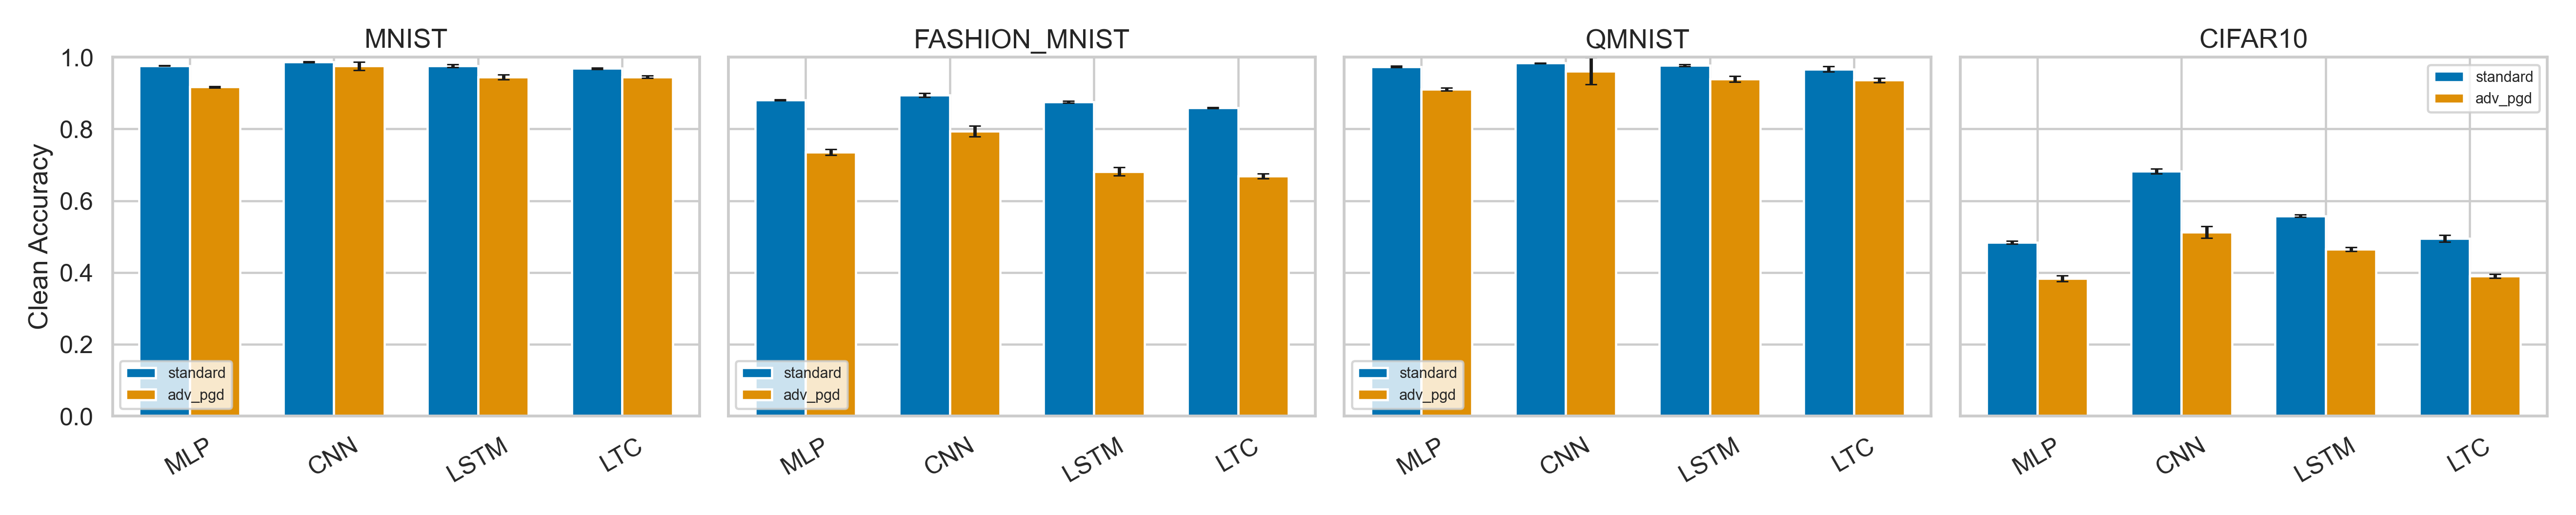
\includegraphics[width=0.82\textwidth]{figures/clean_accuracy_by_defense_seaborn.png}
\caption{Clean accuracy by dataset, architecture, and defense (seaborn rendering).}
\label{fig:clean-bars}
\end{figure*}

\subsection{White-box PGD Robustness}
Table~\ref{tab:pgdauc} reports PGD AUC. Under standard training, LTC is often similar or lower than LSTM. Under adversarial training, robustness increases substantially for all model families.

\begin{table*}[t]
\centering
\caption{PGD AUC (higher is better; mean across five seeds).}
\label{tab:pgdauc}
\small
\begin{tabular}{llrrrr}
\toprule
Dataset & Defense & MLP & CNN & LSTM & LTC \\
\midrule
MNIST & Standard & 0.1421 & 0.3746 & 0.1611 & 0.1453 \\
MNIST & Adv-PGD & 0.5530 & 0.7462 & 0.6717 & 0.7124 \\
Fashion-MNIST & Standard & 0.1207 & 0.1022 & 0.1247 & 0.1165 \\
Fashion-MNIST & Adv-PGD & 0.4745 & 0.5751 & 0.4665 & 0.4566 \\
QMNIST & Standard & 0.1423 & 0.3609 & 0.1699 & 0.1465 \\
QMNIST & Adv-PGD & 0.5530 & 0.7298 & 0.6744 & 0.7037 \\
CIFAR-10 & Standard & 0.1576 & 0.1294 & 0.1532 & 0.1096 \\
CIFAR-10 & Adv-PGD & 0.2664 & 0.3318 & 0.3115 & 0.2632 \\
\bottomrule
\end{tabular}
\end{table*}

\begin{figure*}[t]
\centering
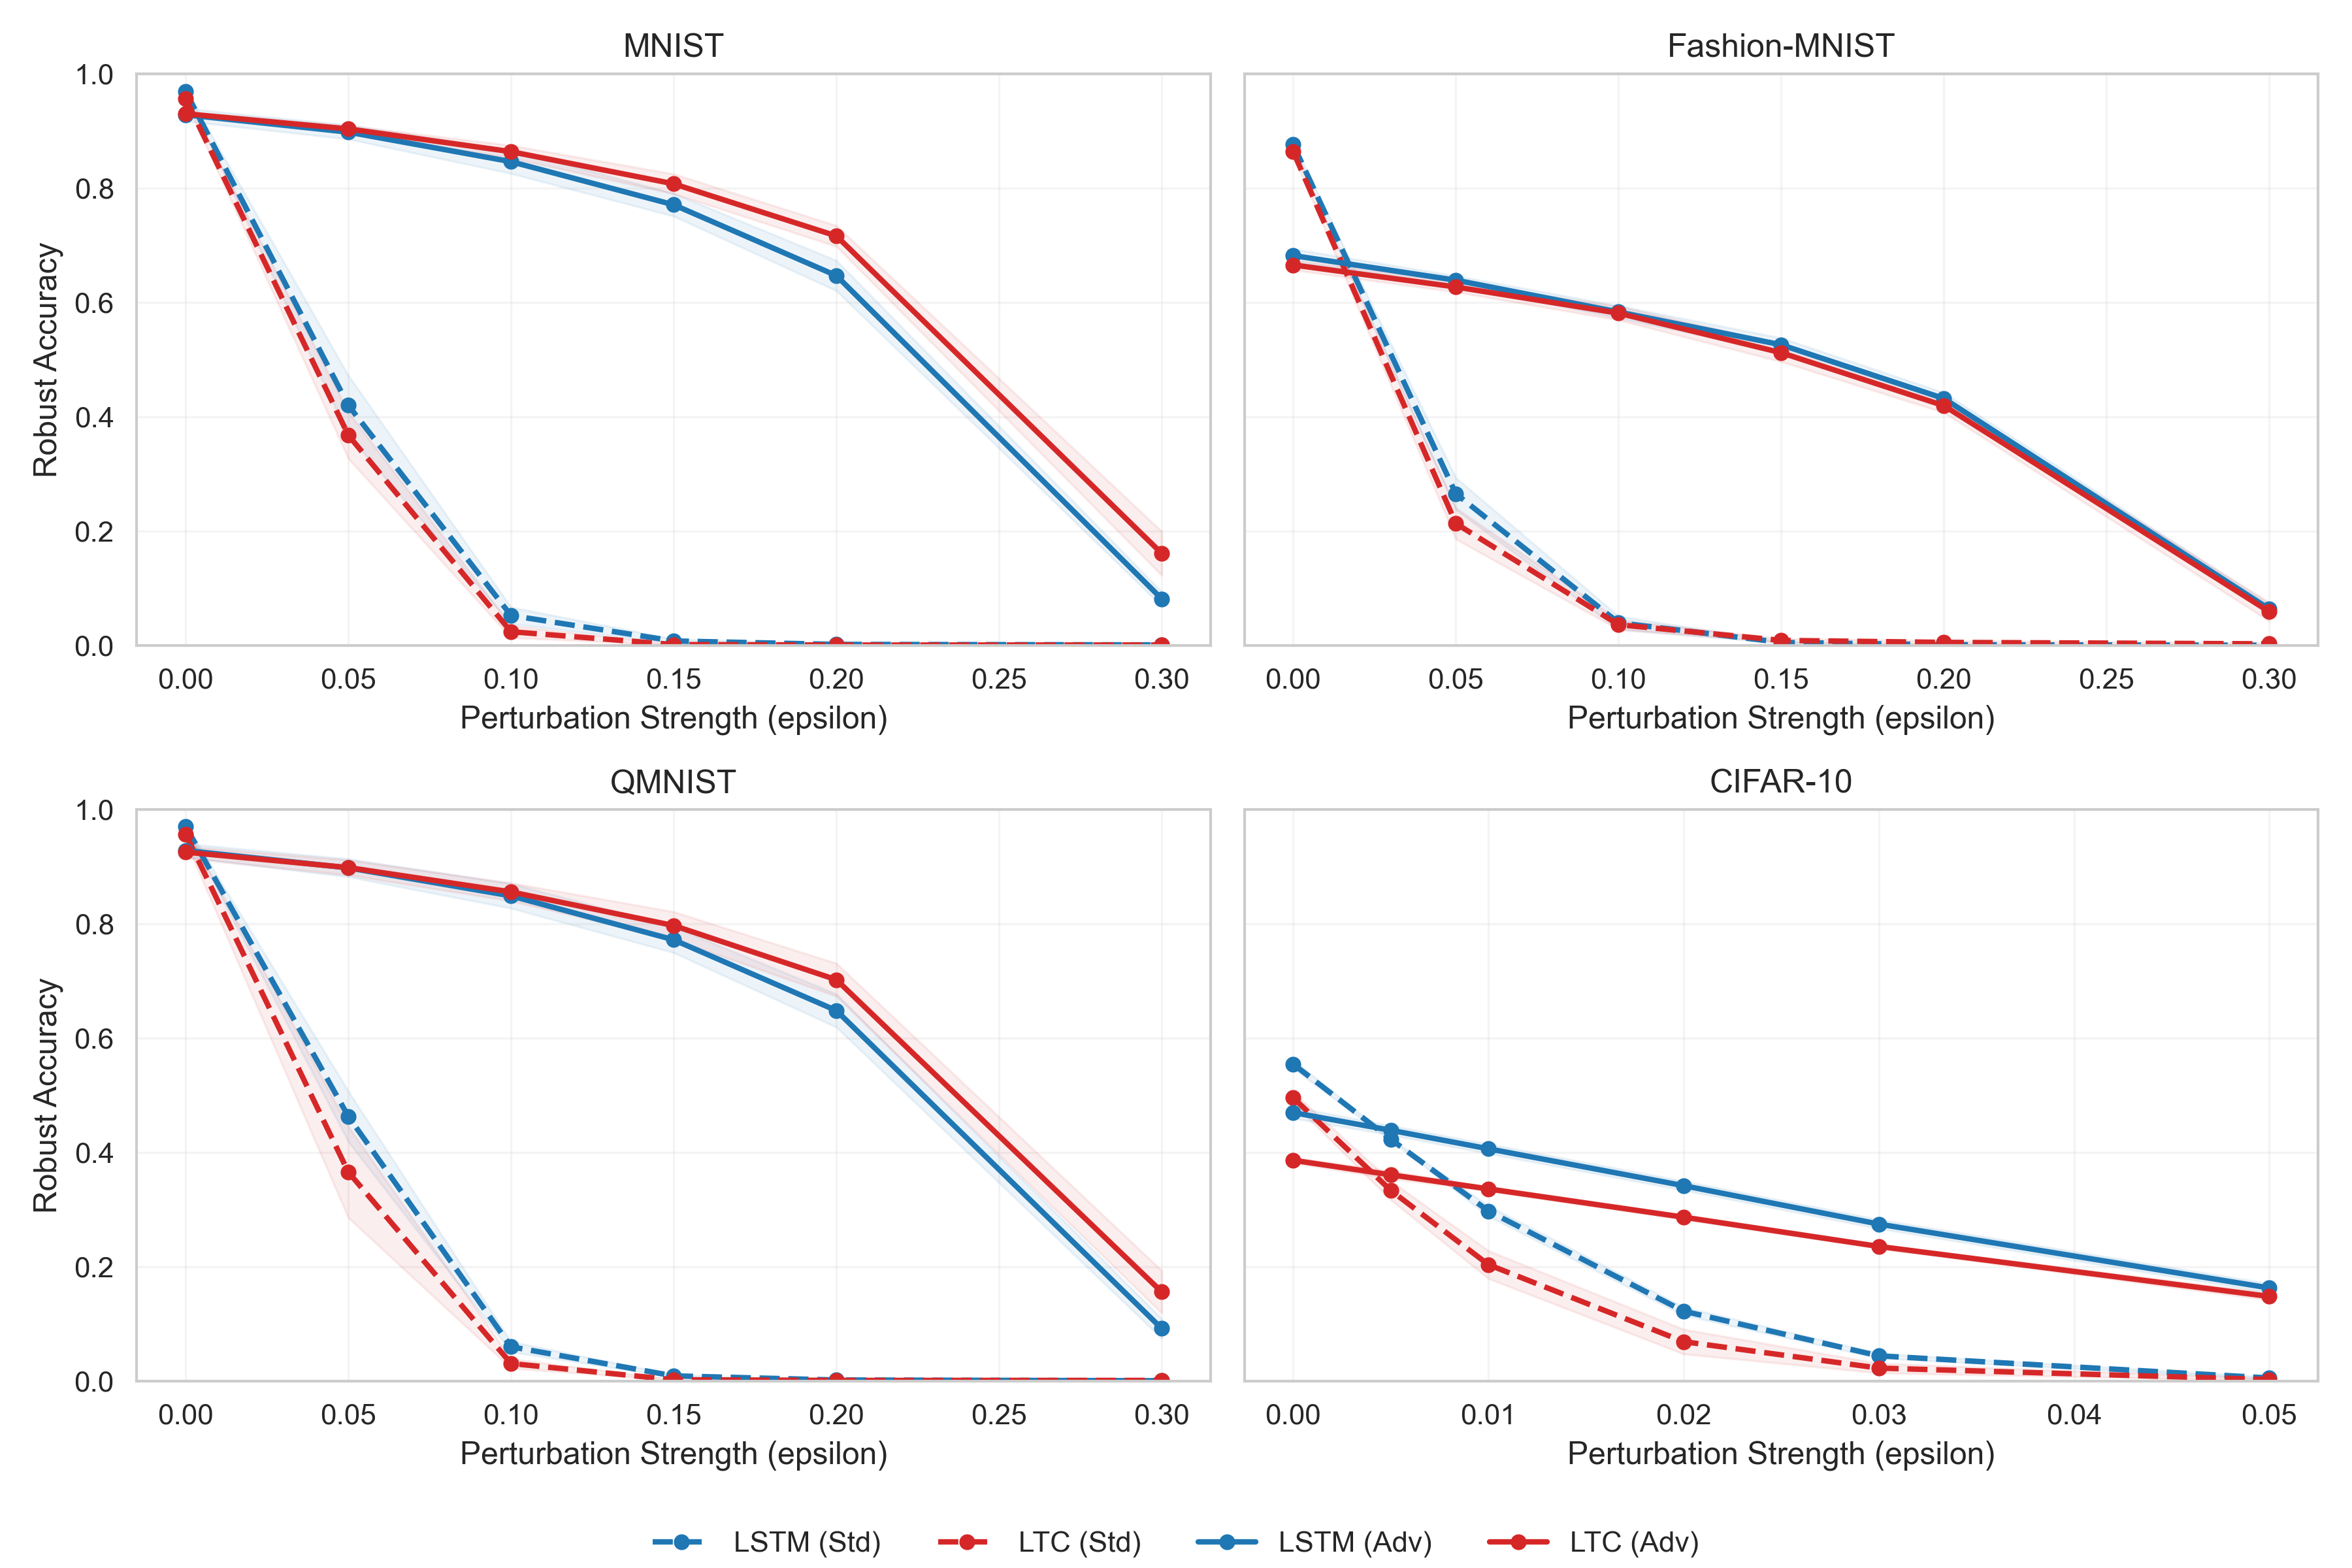
\includegraphics[width=\textwidth]{figures/fig_ltc_lstm_pgd_curves.png}
\caption{PGD robust-accuracy curves comparing LSTM and LTC under standard and adversarial training. Dashed lines: standard training. Solid lines: adversarial training.}
\label{fig:lstm-ltc-pgd}
\end{figure*}

\subsection{Direct LTC-LSTM Contrast}
Figure~\ref{fig:summary-bars} (left) summarizes LTC-LSTM PGD AUC deltas with bootstrap 95\% CIs. The sign changes across datasets/training regimes:
\begin{itemize}
\item Standard: LTC is lower on all four datasets.
\item Adv-PGD: LTC is higher on MNIST and QMNIST, lower on Fashion-MNIST and CIFAR-10.
\end{itemize}
This mixed pattern does not support a universal intrinsic robustness advantage for LTC.

\subsection{Transferability Asymmetry}
Cross-model transfer remains substantial. Figure~\ref{fig:summary-bars} (right) reports
the difference between cross-transfer accuracies for LSTM-crafted attacks on LTC
and LTC-crafted attacks on LSTM.
Negative values imply stronger transfer from LTC-crafted examples into LSTM. The asymmetry direction is dataset-dependent, indicating partially overlapping but non-identical adversarial subspaces.

\begin{figure*}[t]
\centering
\begin{subfigure}[t]{0.49\textwidth}
  \centering
  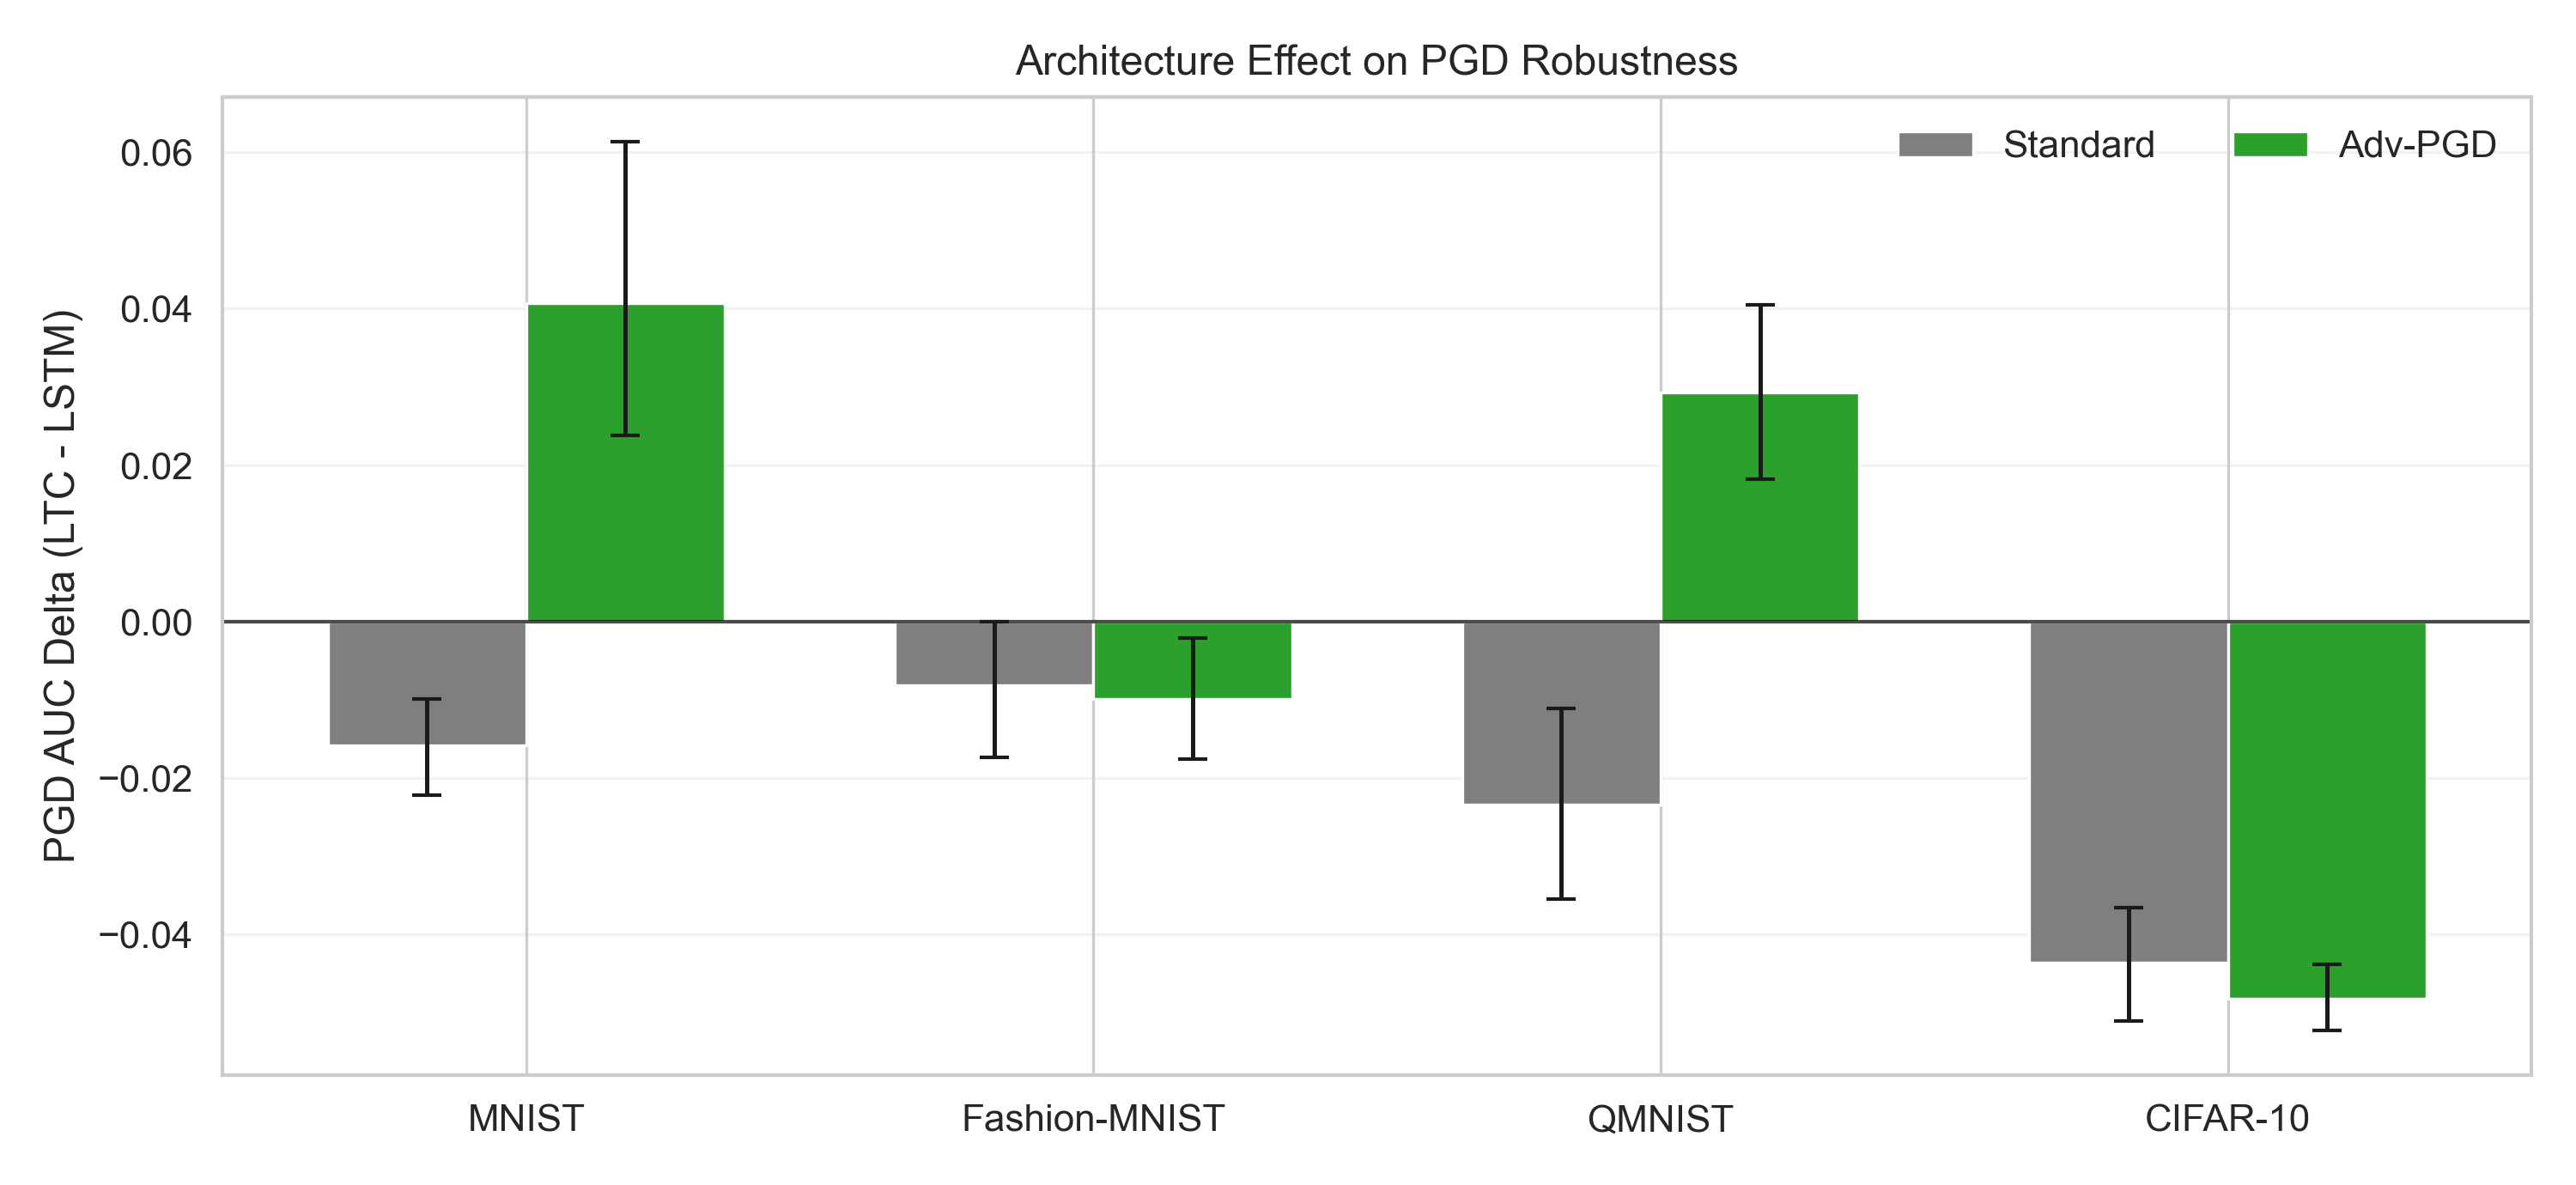
\includegraphics[width=\textwidth]{figures/fig_auc_delta_ltc_minus_lstm.png}
  \caption{PGD AUC delta (LTC - LSTM) with bootstrap 95\% CIs.}
\end{subfigure}
\hfill
\begin{subfigure}[t]{0.49\textwidth}
  \centering
  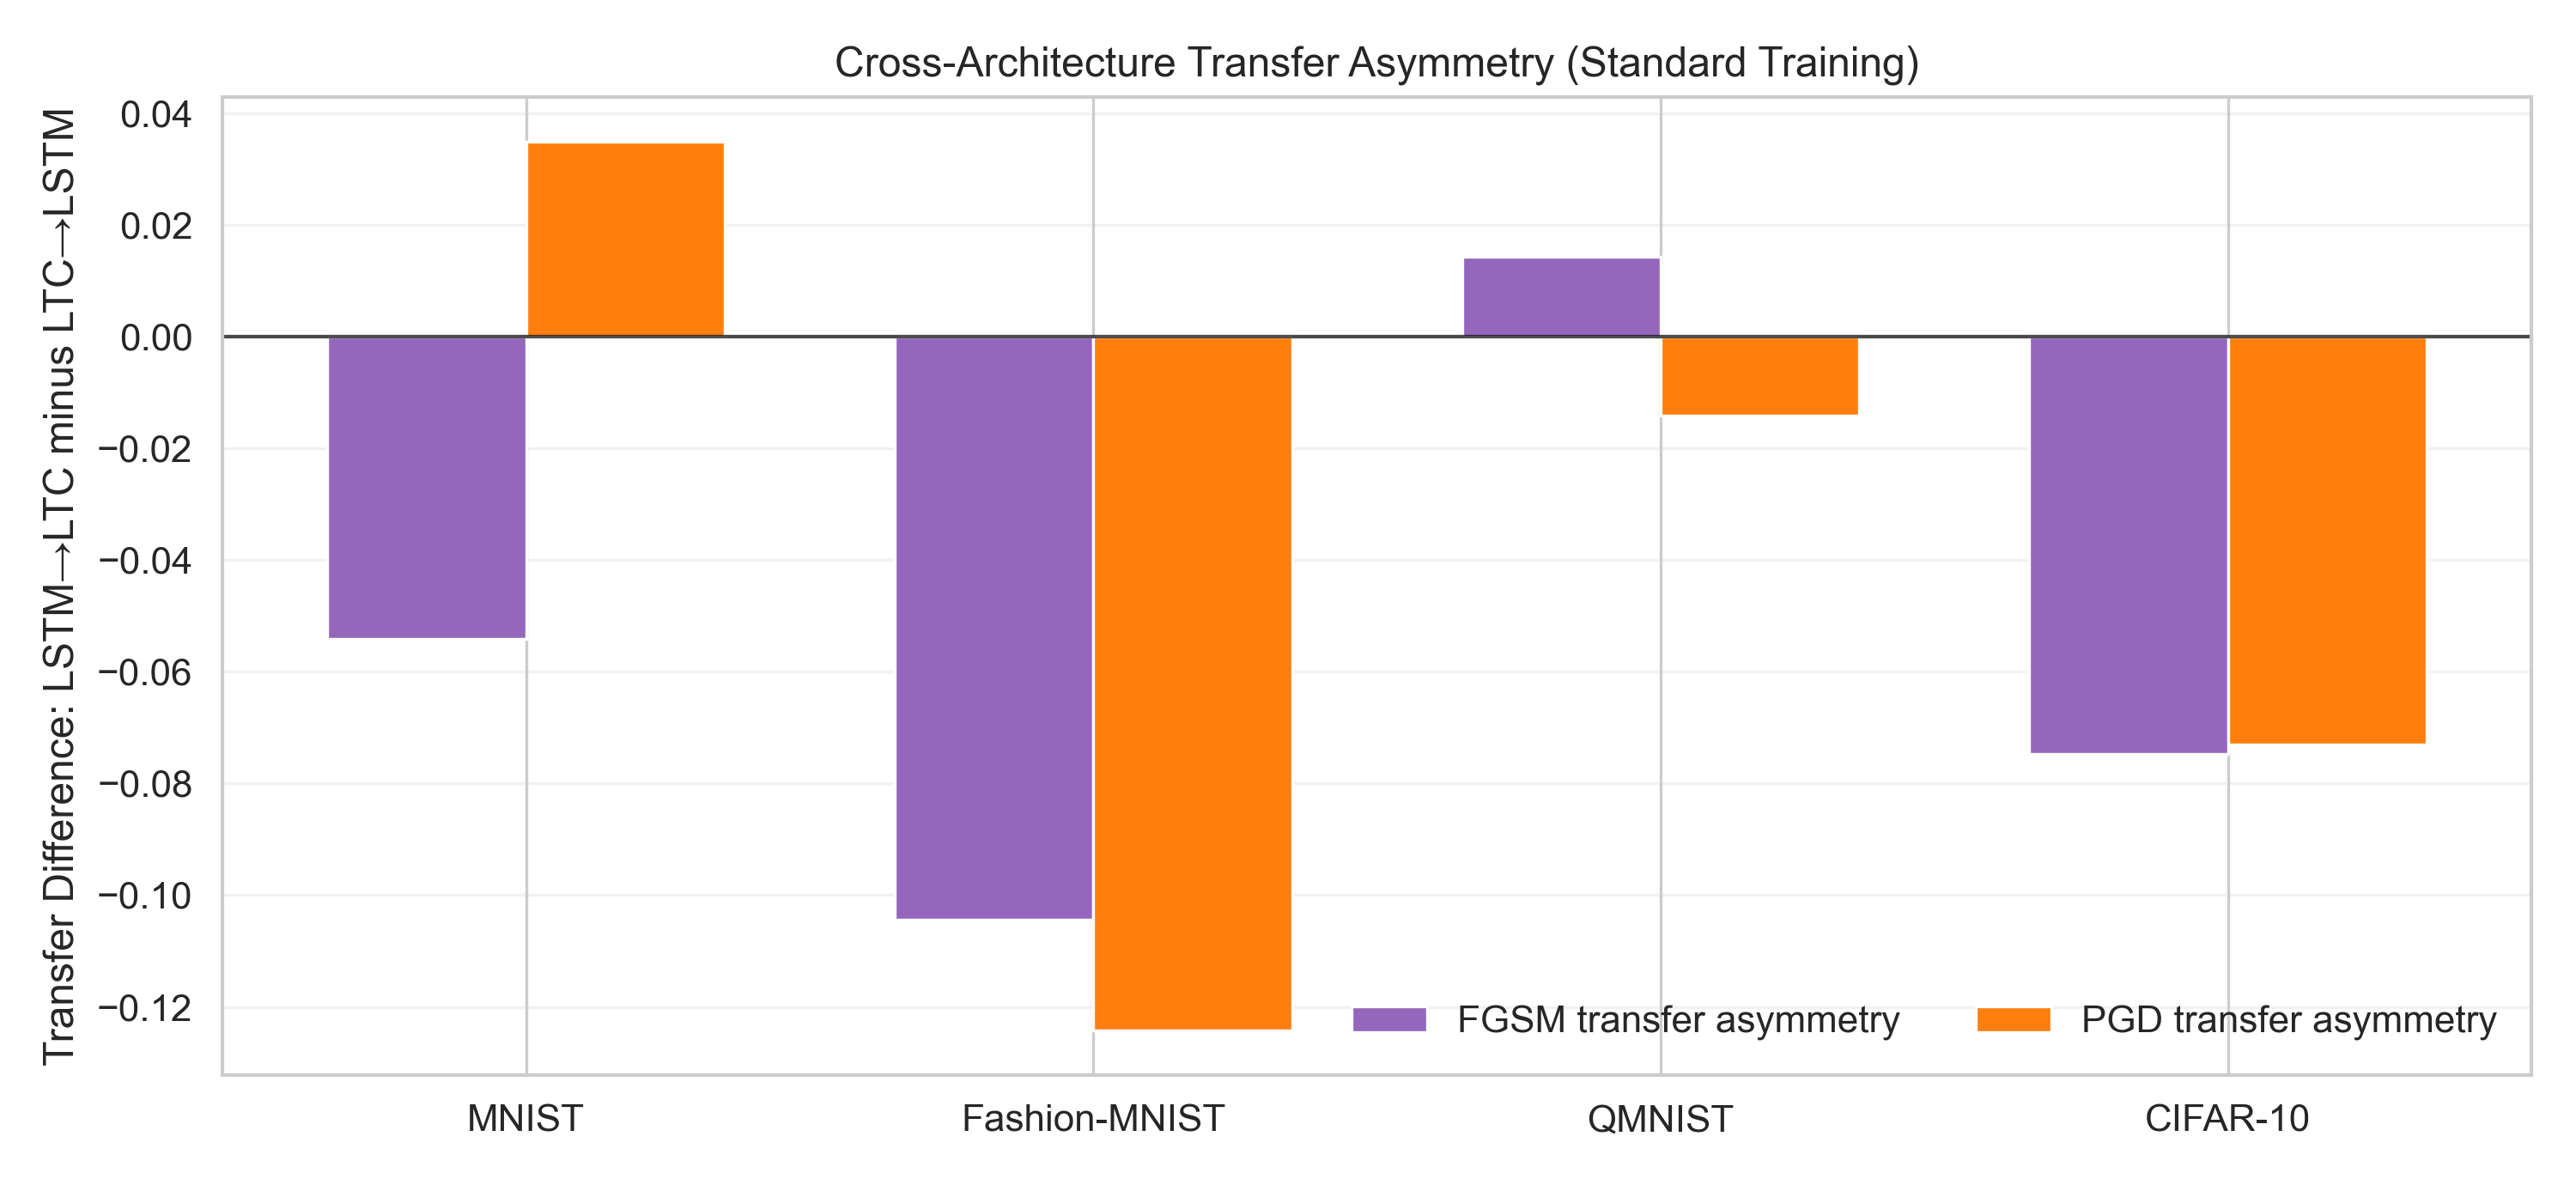
\includegraphics[width=\textwidth]{figures/fig_transfer_asymmetry.png}
  \caption{Transfer asymmetry: $LSTM \to LTC$ minus $LTC \to LSTM$.}
\end{subfigure}
\caption{Summary comparisons for architecture effect and transfer asymmetry under standard/adversarial conditions.}
\label{fig:summary-bars}
\end{figure*}

\section{Discussion}
The strongest empirical effect is from \emph{training objective}, not architecture family. Adversarial training raises PGD robustness broadly, while switching from LSTM to LTC alone does not reliably improve robustness. This result aligns with concerns that apparent robustness can reflect evaluation weaknesses or gradient obfuscation \citep{athalye2018obfuscated}; accordingly, this benchmark uses strong white-box first-order attacks and explicit contamination controls.

\section{Limitations}
This study focuses on first-order attacks (FGSM/PGD). Additional evaluation with AutoAttack/CW and certified methods would further strengthen claims. CIFAR-10 models are intentionally compact for tractable multi-seed sweeps; larger backbones may shift absolute accuracy while likely preserving the architecture-vs-training conclusion.

\section{Conclusion}
Across four datasets, four architecture classes, two defenses, and five seeds per condition, LTC does not demonstrate a consistent intrinsic adversarial robustness advantage over LSTM under standard training. Robust optimization remains the dominant lever.

\clearpage
\bibliographystyle{unsrtnat}
\bibliography{references}

\end{document}
